\section{Grundlagen}

\subsection{Eingesetzte Technologien und Programme}
Im Folgenden werden Technologien und Programme vorgestellt, die während des Projektes eingesetzt wurden.

Unter den Technologien, die in dem Projekt Verwendung finden, befindet sich für die programmatischen Implementierungsarbeiten die Hochsprache Java sowie deren Standardbibliothek Swing zur GUI Entwicklung. Als integrierte Entwicklungsumgebung wird Eclipse Neon eingesetzt. Im Bereich der Datenauswertung und der grafischen Aufbereitung von Daten kommen die Standardprogramme Excel, Word und Visio, als Teil der Microsoft Office Suite, zum Einsatz. Für alle datenbankspezifischen Tätigkeiten wird die Datenbanksprache Oracle SQL mit dem Oracle eigens entwickelten Datenbankmanagement Programm SQL-Developer verwendet.

Oracle SQL ist die meistverwendete Datenbanksprache und wird überall dort genutzt, wo es darum geht Datenbankstrukturen und Daten mittels Programme zu erreichen. Eine Erweiterung dieser Datenbanksprache ist PL/SQL das dazu entwickelt wurde Unterprogramme mit Parametrisierung und Rückgabewerten in Form von Funktionen und Prozeduren auszuführen und als separate Programme innerhalb eines Datenbankschemas zu speichern. Das Datenbankmanagement Programm SQL-Developer vom Hersteller Oracle ist speziell für diese Ausführung der Datenbanksprache entwickelt worden. Darüber hinaus bietet es die Möglichkeit die Datenbankstrukturen zu verwalten und zu erweitern. Durch die integrierte Ausgabekonsole lassen sich selektierte Daten direkt in einer tabellarischen Ansicht darstellen. Mit der eingebetteten Autovervollständigung und Syntax Überprüfung lassen sich relativ einfach und unkompliziert verschachtelte Datenbankabfragen erstellen und ausführen.

\subsection{Software-Ergonomie}
\begin{quote}
    Die Software-Ergonomie hat es sich zur Aufgabe gemacht, die Merkmale benutzer- und aufgebengerechter Software zu erforschen und konstruktive Verfahren sowie Softwareunterstützungen für den Prozeß der Gestaltung von Benutzungsschnittstellen zu entwickeln. Ihr zentrales Anliegen ist die Optimierung des Zusammenspiels aller Komponenten der Arbeitssituation von Computerbenutzern: Mensch, Aufgabe, Technik und organisatorischer Rahmen. \citep{Maass1993}
  \end{quote}
Die relativ allgemeine aber trotzdem sehr treffende Definition von Software-Ergonomie wurde durch die Authorin Dr. Susanne Maaß 1993 veröffentlicht.

Zunächst soll im Folgenden der Begriff der Software-Ergonomie genauer erläutert werden. Anschließend werden Begriffe, die in einem direktem Zusammenhang mit der Software-Ergonomie stehen, erklärt und abgegrenzt. Darauffolgend werden verschiedene Normen, Gesetze, Verordnungen und zuletzt sogenannte Usability Heuristics, die in der Vergangenheit entworfen wurden, vorgestellt.

\subsubsection{Begriffsdefinition}
Software-Ergonomie ist die \glqq ability of a software system to interact easily and effectively with the user in order to fulfil his/her needs and expectations\grqq{} \citep[4]{Oppermann1988einfuehrung}, also die Fähigkeit einer Software einfach und effektiv mit einem Benutzer zu interagieren und dabei dessen Anforderungen und Erwartungen zu erfüllen. Das Ergebnis aus der Software-Ergonomie ist die Usability also die Gebrauchstauglichkeit einer Software. Sie ist besonders dort wichtig, wo Menschen mit Maschinen über Schnittstellen arbeiten \citep[vgl.][]{usabilityDe}. Die Usability ist der Zusammenschluss von Effektivität, Effizienz und Zufriedenheit. Effektivität beschreibt die Erreichung und das Ausmaß von Zielen. Effizienz stellt den Aufwand für die Erledigung des Ziels dar. Die Zufriedenheit spiegelt subjektive Faktoren wie \glqq joy of use\grqq{}, \glqq look and feel\grqq{} und \glqq motivation and fun\grqq{} wider \citep[vgl.][]{Holzinger2011human}. Die Zufriedenheit wird auch als User Experience (UX) bezeichnet, die als Erweiterung der Gebrauchstauglichkeit gesehen wird, da sie ästhetische und emotionale Faktoren mit einbezieht \citep[vgl.][]{usabilityDe}. Die Software-Ergonomie gehört neben der Hardware-Ergonomie und Organisations-Ergonomie zu den drei ergonomischen Disziplinen. Auch die Software-Ergonomie selbst lässt sich in drei weitere Bereiche aufteilen: Korrektheits-Ergonomie, Funktionalitäts-Ergonomie und Schnittstellen-Ergonomie \citep[vgl.][]{Oppermann1988einfuehrung}.

\subsubsection{Gestaltgesetze}
In der Vergangenheit wurden durch interdisziplinären Ansätze verschiedene Gestaltgesetze entwickelt, die als Hilfestellung bei der Entwicklung von grafischen Benutzerschnittstellen dienen sollen. Gestalt bedeutet dabei soviel wie automatische Zusammenfassung bzw. Gruppierung von Objekten \citep[vgl.][59]{Dahm2006}. Bei der Beobachtung von Bildern und Grafiken werden unterbewusst gewisse Muster und Gruppen aus einzelnen Elementen gebildet. Diese Muster und Gruppen lassen sich in einige wichtige Gestaltgesetze abstrahieren, die schon 1923 von drei Forschern beobachtet und niedergeschrieben wurden. Die Gestaltsgesetze können für das Gruppieren und Abgrenzen von Elementen untereinander verwendet werden, um eine höhere Ästhetik bzw. Übersichtlichkeit zu erzielen. Im Folgenden werden sechs wichtige Gestaltgesetze vorgestellt.

\textbf{Gesetz der Ähnlichkeit}

Wie in Abbildung \ref{fig:aehnlichkeit} zu sehen ist, werden ähnliche Objekte zusammengefasst. Für den Betrachter gruppieren sich die grauen und blauen Elementen und er nimmt Spalten wahr.
\begin{figure}[H]
  \centering
  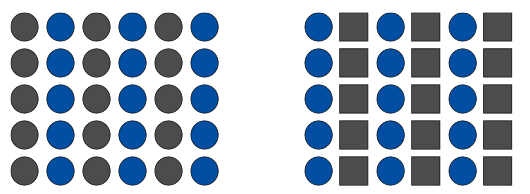
\includegraphics[scale=1]{img/gesetz_der_Aehnlichkeit.PNG}
  \caption{Ähnliche Objekte werden zusammengefasst.}
    \caption*{\textbf{Quelle:} \citep{Dahm2006}}
  \label{fig:aehnlichkeit}
\end{figure}
Für die Ähnlichkeit sind die Farbe, die Helligkeit, die Form, das Muster und noch weitere Kriterien von Bedeutung \citep[vgl.][59f]{Dahm2006}. Je mehr Kriterien Elemente gemeinsam haben, desto höher ist dessen Ähnlichkeit und desto eher werden Elemente als Gruppe gesehen \citep[vgl.][]{HTMLSeminarDe}.

\textbf{Gesetz der Nähe}

Das Gesetz der Nähe beschreibt die Zusammengehörigkeit von Elementen durch ihre Nähe zueinander.
\begin{figure}[H]
  \centering
  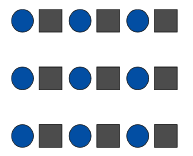
\includegraphics[scale=1]{img/gesetz_der_Naehe.PNG}
  \caption{Abstände zwischen Objekten erzeugen eine Zusammengehörigkeit.}
    \caption*{\textbf{Quelle:} \citep{Dahm2006}}
  \label{fig:naehe}
\end{figure}
In der Abbildung \ref{fig:naehe} ist zu erkennen, dass die Elemente trotz unterschiedlicher Formen und Farben  nicht als Spalten, sondern als Zeilen, wahrgenommen werden. Dieser Effekt resultiert aus dem dominanten Merkmal der Nähe von Objekten. Die Nähe erzielt bei der Anordnung von Elementen einen noch stärkeren Effekt als die Ähnlichkeit \citep[vgl.][60]{Dahm2006}.

\textbf{Prägnanz oder Gute Gestalt}

\begin{figure}[H]
  \centering
  
\includegraphics[scale=1]{img/gesetz_der_Praegnanz_oder_der_Guten_Gestalt.PNG}
  \caption{Prägnanz oder Gute Gestalt.}
    \caption*{\textbf{Quelle:} \citep{Dahm2006}}
  \label{fig:praegnanzOderGuteGestalt}
\end{figure}
Das Gesetz der Prägnanz oder der Guten Gestalt besagt das zusammengesetzte Objekte zuerst meist als einzelne einfache Objekte gesehen werden. Die Abbildung \ref{fig:praegnanzOderGuteGestalt} ist ein Beispiel dafür, das unsere kognitiven Fähigkeiten dazu in der Lage sind komplexere Objekte in getrennte geometrische Formen zu zerlegen. Dabei sieht man in der Abbildung eine Ellipse und ein Dreieck anstatt eines konstruierten Objektes. Diese Fähigkeit ist schon auf eine frühe Vergangenheit zurückzuführen, in der wir in dunklen Umgebungen bedrohliche Tiere vom restlichen Hintergrund trennen mussten um zu überleben \citep[vgl.][61]{Dahm2006}.

\textbf{Fortsetzung und Ergänzung}

Das Gesetz besagt das gleiche und ähnliche Objekte die Gestalt einer Linie annehmen können und diese Linie getrennt von anderen Objekten wahrgenommen wird.
\begin{figure}[H]
  \centering
  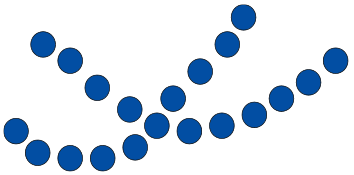
\includegraphics[scale=1]{img/gesetz_der_Fortsetzung_und_Ergaenzung.PNG}
  \caption{Gesetz der Fortsetzung und Ergänzung.}
    \caption*{\textbf{Quelle:} \citep{Dahm2006}}
  \label{fig:fortsetzungUndErgaenzung1}
\end{figure}
Als Beispiel dient die Abbildung \ref{fig:fortsetzungUndErgaenzung1}, in der zwei gekrümmte Linien durch die Aneinanderreihung von mehreren Kreisen zu erkennen sind. Interessant ist, dass die beiden Linien als sich schneidende gekrümmte Linien gesehen werden und nicht als geknickte Linien die lediglich in einem Punkt identisch sind oder als vier von einem Punkt weglaufende Linien. Dieser Effekt tritt auch immer dann auf, wenn Objekte durch im Vordergrund liegende Objekte unterbrochen werden aber trotzdem vollständig wahrgenommen.
\begin{figure}[H]
  \centering
  
\includegraphics[scale=1]{img/gesetz_der_Fortsetzung_und_Ergaenzung2.PNG}
  \caption{Gesetz der Fortsetzung und Ergänzung als optische Täuschung.}
    \caption*{\textbf{Quelle:} \citep{Dahm2006}}
  \label{fig:fortsetzungUndErgaenzung2}
\end{figure}
Der Effekt der Fortsetzung wird in der oberen Abbildung \ref{fig:fortsetzungUndErgaenzung2} nochmal deutlicher. Hier werden bei der linken Abbildung zwei angefangene Objekte zu jeweils einem Dreieck ergänzt. Ebenso auf der rechten Seite, dort wird alleine durch die Andeutung von vier Ecken ein vollständiges blaues Quadrat wahrgenommen \citep[vgl.][61f]{Dahm2006}.

\textbf{Gemeinsames Schicksal}

Aus einer Vielzahl von Objekten, lassen sich diejenigen zusammenfassen dessen gleichförmige Bewegung sich gleicht.
\begin{figure}[H]
  \centering
  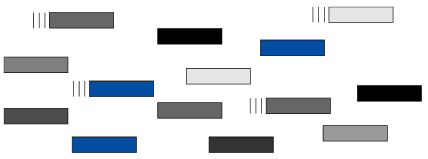
\includegraphics[scale=1]{img/gesetz_des_gemeinsamen_Schicksals.PNG}
  \caption{Zusammengehörigkeit von Objekten durch ihr gemeinsames Schicksal.}
    \caption*{\textbf{Quelle:} \citep{Dahm2006}}
  \label{fig:gemeinsamesSchicksal}
\end{figure}
Dieser Effekt tritt am stärksten bei bewegten Objekten auf und wird trotz unterschiedlicher Farben und Anordnungen wahrgenommen. In Abbildung \ref{fig:gemeinsamesSchicksal} wird der Effekt, der sich \glqq Gemeinsames Schicksal\grqq{} nennt, versucht darzustellen \citep[vgl.][62]{Dahm2006}.

\textbf{Gesetz der Vertrautheit}

Das Gesetz der Vertrautheit beschreibt ein Phänomen, bei dem bekannte Formen immer wieder erkannt werden auch wenn sie aus einzelnen simplen Objekten zusammengesetzt werden.
\begin{figure}[H]
  \centering
  
\includegraphics[scale=0.7]{img/gesetz_der_Vertrautheit.PNG}
  \caption{Vertraute Formen bleiben beim Betrachter erhalten.}
  \caption*{\textbf{Quelle:} \citep{Dahm2006}}
  \label{fig:vertrautheit}
\end{figure}
In Abbildung \ref{fig:vertrautheit} sieht der Betrachter auf den ersten Blick viele wahllos verstreute schwarze Flecken auf einem weißen Hintergrund. Wird nun die Erfahrung des Betrachters mit Informationen zu diesem Bild angereichert, wird er zukünftig diese Erfahrungen automatisch immer wieder abrufen ohne diese unterdrücken zu können. In dieser Abbildung ist in der rechten Bildhälfte ein herabschauender Dalmatiner zu sehen. Von vielen Personen wird der Dalmatiner durch bloßes hinschauen nicht wahrgenommen. Sobald der Betrachter einmal den Dalmatiner entdeckt hat, wird er nie wieder nur wahllose Flecken sehen können. \citep[vgl.][63f]{Dahm2006}.

\subsubsection{Normen, Gesetze und Verordnungen}
Neben den Gesetzen zur Gestaltung und Anordnung von Elementen gibt es eine Vielzahl von Normen, Gesetzen und Verordnungen die sich aus verschiedensten Arbeitsgruppen, Institutionen und Gremien entwickelt haben. Ein Grund für ihre Existenz sind die zunehmende Bedeutung von Benutzerschnittstellen und deren Gebrauchstauglichkeit und gleichzeitig auch die steigende Komplexität von Benutzerschnittstellen. Die Normen, also Anweisungen, einer höheren Instanz, für das Verhalten bei gewissen Tätigkeiten, Situationen, o.Ä. \citep[vgl.][]{duden}, dienen der Unterstützung bei der Entwicklung von einheitlichen und benutzerfreundlichen Benutzerschnittstellen. Gesetze und Verordnungen werden vom Gesetzgeber als Vorgaben an die Software-Ergonomie gestellt.

\textbf{Normen}

Die Software-Ergonomie Norm \gls{DIN} \gls{EN} \gls{ISO} 9241 wurde in ihrer ersten Auflage 1996 veröffentlicht. Seitdem sind die Anforderungen und technischen Möglichkeiten immer weiter gewachsen. In dem Zuge wurde die Norm 2008 in einer überarbeiteten Fassung herausgegeben. Dabei wurden konkretere Beispiele und Empfehlungen vervielfältigt, der Nutzungskontext, der zuvor nur mit dem Blick auf PC'S gerichtet war, erweitert und zusätzlich andere Normen mit einbezogen \citep[vgl.][]{schneider2008}.

Der Begriff Gebrauchstauglichkeit wird in der Norm 9241-110 mit den drei Merkmalen Effektivität, Effizienz und Zufriedenheit aus der Norm 9241-11 definiert. Zudem wird im Kapitel 6 des Normteils 110 (ehemals Teil 10) die Verbindung der sieben Gestaltungsgrundsätze für ergonomische Benutzerschnittstellen (s. Tabelle \ref{tab:siebenGrundprinzipien}), aus ISO 9241-110 und ISO 9241-12, zu der Gebrauchstauglichkeit aus ISO 9241-11 hergestellt. Die Anwendung der sieben Grundsätze unterstützt die Gebrauchstauglichkeit \citep[vgl.][Kap. 6]{ISO9241-110}.

Wie in der Tabelle \ref{tab:siebenGrundprinzipien} zu erkennen ist, wurden die einzelnen Grundprinzipien in ihren Beschreibungen möglichst generisch formuliert. Ein Grund dafür ist, dass die Grundsätze unabhängig vom betrachtenden Softwaresystem angewandt werden sollen. Die Grundsätze können bei der Konzeption, Analyse und Bewertung von Dialogen angewandt werden, sollen aber keine Vorgaben an die Entwicklung von interaktiven Systemen stellen \citep[vgl.][Kap. 4.1]{ISO9241-110}.

\begin{center}
\begin{longtable}{|p{5.1cm}|p{9.5cm}|} 
\hline
\textbf{Grundprinzip} & \textbf{Beschreibung} \\ \hline
Aufgabenangemessenheit & Ein interaktives System ist aufgabenangemessen, wenn es den Benutzer unterstützt, seine Arbeitsaufgabe zu erledigen, d.h., wenn Funktionalität und Dialog auf den charakteristischen Eigenschaften der Arbeitsaufgabe basieren, anstatt auf der zur Aufgabenerledigung eingesetzten Technologie. \\ \hline
Selbstbeschreibungsfähigkeit & Der Dialog ist in dem Maße selbstbeschreibungsfähig, in dem für den Benutzer zu jeder Zeit offensichtlich ist, in welchem Dialog, an welcher Stelle im Dialog er sich befindet, welche Handlungen unternommen werden können und wie diese ausgeführt werden können. \\ \hline
Erwartungskonformität & Ein Dialog ist erwartungskonform, wenn er den aus dem Nutzungskontext heraus vorhersehbaren Benutzerbelangen sowie allgemein anerkannten Konventionen entspricht. \\ \hline
Lernförderlichkeit & Ein Dialog ist lernförderlich, wenn er den Benutzer beim Erlernen der Nutzung des interaktiven Systems unterstützt und anleitet. \\ \hline
Steuerbarkeit & Ein Dialog ist steuerbar, wenn der Benutzer in der Lage ist, den Dialogablauf zu starten sowie seine Richtung und Geschwindigkeit zu beeinflussen bis das Ziel erreicht ist. \\ \hline
Fehlertoleranz & Ein Dialog ist fehlertolerant, wenn das beabsichtigte Arbeitsergebnis trotz erkennbar fehlerhafter Eingaben entweder mit keinem oder mit minimalem Korrekturaufwand seitens des Benutzers erreicht werden kann. Fehlertoleranz wird mit den Mitteln erreicht: 
\begin{itemize}\itemsep0pt
  \item Fehlererkennung und -vermeidung (Schadensbegrenzung)
  \item Fehlerkorrektur oder
  \item Fehlermanagement, um mit Fehlern umzugehen, die sich ereignen.
\end{itemize} \\ \hline
Individualisierbarkeit & Ein Dialog ist individualisierbar, wenn Benutzer die Mensch-System-Interaktion und die Darstellung von Informationen ändern können, um diese an ihre individuellen Fähigkeiten und Bedürfnisse anzupassen.\\ \hline
\caption{Die sieben Grundprinzipien der Dialoggestaltung in Anlehnung an \citep[]{ISO9241-110}.}
\label{tab:siebenGrundprinzipien}
\end{longtable}
\end{center}
Bei der konkreten Umsetzung sollten zunächst Merkmale der zukünftigen Benutzer, Arbeitsaufgaben, Arbeitsumgebung aber auch die zur Verfügung stehenden Technologien analysiert werden, um herauszufinden welcher dieser Prinzipien im vorliegenden Kontext geeignet sind \citep[vgl.][]{Figl2010}. 

Im Abschnitt 12 der ISO Norm 9241 werden die charakteristischen Eigenschaften der Informationsdarstellung, d.h. Klarheit, Unterscheidbarkeit, Kompaktheit, Konsistenz, Erkennbarkeit, Lesbarkeit und Verständlichkeit als unterstützendes Bindeglied für die sieben Grundsätze aus Teil 110 definiert. Insbesondere die Selbstbeschreibungsfähigkeit und Erwartungskonformität einer Benutzerschnittstelle können, durch die Eigenschaften der ISO 9241-12, positiv beeinflusst werden. Insgesamt sind die Teile 110, 11 und 12 der ISO Norm 9241 eng miteinander verkettet und können positive aber auch negative Effekte aufeinander ausüben \citep[vgl.][Kap. 6]{ISO9241-110}. Die Wirkungsrichtungen der einzelnen Teile werden in Abbildung \ref{fig:beziehungIsoNormen} noch einmal genauer verdeutlicht.
\begin{figure}[H]
  \centering
  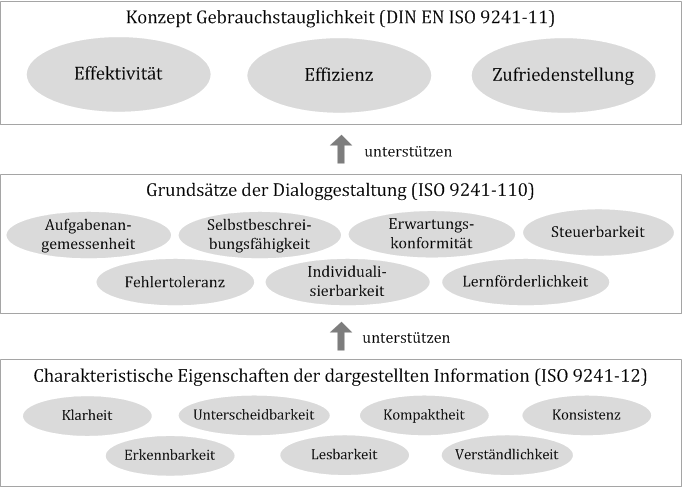
\includegraphics[scale=0.86]{img/Beziehung_ISO9241_ISO9241-11_ISO9241-12.png}
  \caption{Beziehung zwischen ISO 9241, ISO 9241-11 und ISO 9241-12 in Anlehnung an \citep[]{ISO9241-110}.}
  \caption*{\textbf{Quelle:} eigene Darstellung}
  \label{fig:beziehungIsoNormen}
\end{figure}
Eine weitere Norm im Bereich der Software-Ergonomie auf die im Abschnitt 3.6 in der ISO 9241-110 Norm verwiesen wird, ist die DIN EN ISO 13407 (Benutzerorientierte Gestaltung interaktiver Systeme). Diese Norm ist als Ergänzung des Teils 110, im Bereich des Projektmanagements und der Vorgehensweisen, anzusehen \citep[vgl.][58]{schneider2008}.

\textbf{Gesetze und Verordnungen}

Die \gls{ArbStaettV} ist ein Gesetz das anstelle der vorherigen Arbeitsschutzverordnung am 3. Dezember 2016 in Kraft getreten ist. Die \gls{ArbStaettV} hat als Ziel Beschäftigte in Arbeitsstätten vor Arbeitsunfällen und Berufskrankheiten zu schützen. Das Gesetz enthält Mindestvorgaben an die Arbeitsstätten, die zur Sicherheit und zum Gesundheitsschutz der Beschäftigten eingeführt wurden \citep[vgl.][]{BAuA}. 

Ein Zusammenhang des Gesetztes mit dem Thema Ergonomie wird deutlich, wenn man sich den Anlagen Teil 6 des Gesetztes anschaut. Dort lassen sich Maßnahmen und Vorgaben zur Gestaltung von Bildschirmarbeitsplätzen finden. Diese Anforderungen wie zum Beispiel die angemessene Skalierung von Texten und Grafiken oder auch der ausreichende Kontrast von Texten und Grafiken zum Hintergrund, tragen ebenfalls zu den ergonomischen Gesichtspunkten einer gebrauchstauglichen Benutzerschnittstelle bei \citep[vgl.][Anhang: Kap. 6]{ArbStaettV}.

\subsubsection{Heuristiken der Gebrauchstauglichkeit}
Auf dem Gebiet der Usability von Benutzerschnittstellen und der Interaktion mit Schnittstellen, sind der Informatik Professoren Ben Shneidermann und Don Norman und der Usability Berater Dr. Jakob Nielsen, eine renommierte Referenz \citep[vgl.][]{Wong2018}. Mit ihren unzähligen Werken erreichten sie immer wieder, dass ihre Erkenntnisse bis heute als anerkannt gelten und gerne referenziert werden. Diese praktikablen Ansätze und Vorgehensweisen für die Evaluation von ergonomischen Benutzerschnittstellen werden Usability Heuristiken genannt. Heuristiken sind Methoden, die auf überlieferten Verhaltensweisen und Erfahrungen basieren und dabei helfen komplexe Probleme zu lösen \citep[vgl.][]{Heuristik2018}. Im folgenden werden 10 Usability Heuristiken von Dr. Jakob Nielsen vorgestellt.
\begin{itemize}
    \item Das System sollte dem Anwender immer wieder den aktuellen Status mitteilen \citep[vgl.][]{Nielsen1995}.
    \item Die Sprache und Ausdrucksweise des Systems sollte zu dem des Anwenders passen. Dazu zählt auch, dass Informationen in realen und logischen Reihenfolgen dargestellt werden \citep[vgl.][]{Nielsen1995}.
    \item Der Anwender sollte die Möglichkeit haben Aktionen zu widerrufen und erneut auszuführen. Bei kritischen Aktionen sollte erst nach einer Bestätigung der Status eines Dialoges gewechselt werden \citep[vgl.][]{Nielsen1995}.
    \item Die Konventionen für Syntax und Semantik sollten systemweit einheitlich eingehalten werden \citep[vgl.][]{Nielsen1995}.
    \item Das System sollte so konzipiert sein, dass es keine Fehlermeldungen zulässt \citep[vgl.][]{Nielsen1995}.
    \item Wichtige Informationen sollte jederzeit im System einsehbar sein. Hilfen zur Handhabung des Systems sollten leicht zugänglich sein \citep[vgl.][]{Nielsen1995}.
    \item Das System sollte sowohl für erfahrene Anwender als auch für unerfahrene Benutzer konzipiert sein \citep[vgl.][]{Nielsen1995}.
    \item Die Dialoge in einem System sollten immer nur wichtige Informationen anzeigen \citep[vgl.][]{Nielsen1995}.
    \item Fehlermeldungen sollten immer in verständlichen Inhalten für den Anwender dargestellt werden und mögliche Lösungswege vorschlagen \citep[vgl.][]{Nielsen1995}.
    \item Das System sollte eine ausreichende System- und Anwenderdokumentation besitzen. Außerdem sollten Informationen einfach in den Dokumentationen zu finden sein \citep[vgl.][]{Nielsen1995}.
\end{itemize}

Um eine all umfassendere Sicht auf mögliche Strategien und Ziele bei der Entwicklung, Analyse und Konzeption von ergonomischen Benutzerschnittstellen zu bekommen, bieten sich die Ansätze von Dr. Jakob Nielsen an. Eine weitere Auswahl an Usability Heuristiken stellte Ben Shneidermann mit seinen \glqq 8 Golden Rules of Interface Design \grqq{} \citep{Wong2018} auf. Einige der dort genannten Aspekte decken sich mit den Inhalten der 10 Heuristiken von Dr. Jakob Nielsen.

\subsubsection{Nutzen von Software-Ergonomie}
Oftmals sehen Unternehmen zwar den Aspekt der Software-Ergonomie, schrecken aber meist dann zurück wenn zusätzliche Aufwände im Entwicklungsprozess, die im ersten Moment hoch erscheinen, für eine ergonomische Software aufgebracht werden müssten. Langfristig gesehen wird sich jedoch die Software-Ergonomie positiv auf die Produktivität auswirken. Sobald es darum geht Arbeitsabläufe zu optimieren und Zeit zu sparen sind ergonomische Softwaresysteme unabdinglich. Ein gutes Beispiel für die Produktivitätssteigerung durch Software-Ergonomie ist das Service Dialog Center (Call-Center), in dem die Mitarbeiter teilweise durchgehend mit den Software Systemen ihres Unternehmens konfrontiert sind und dessen Produktivität unter anderem davon abhängt wie benutzerfreundlich bzw. ergonomisch die Software auf sie zugeschnitten ist. Dort können schon jeweils wenige Sekunden Ersparnis im Arbeitsablauf eines einzelnen Mitarbeiters, einen großen Mehrwert insgesamt erzielen \citep[vgl.][19]{Pruemper_Harten2007}.

Die Produktivität setzt auch voraus das die Mitarbeiter keinen zu großen Belastungen (physisch und psychisch) ausgesetzt sind. Das heißt sowohl repetitive\footnote{repetitiv = sich wiederholend} Bewegungen der Finger, Hände, Arme und Schultern als auch der Arbeitsablauf und die Arbeitsorganisation sollten möglichst gering bzw. einfach gehalten werden. Zu hohe psychische Belastungen können daraus resultieren, dass zum Beispiel Zeitdruck, ein hoher Konzentrationsaufwand oder zu viele Unterbrechungen in den Arbeitsabläufen auftritt. Diese negativen Effekte gilt es durch eine ergonomische Software möglichst effektiv abzufangen und vorzubeugen \citep[vgl.][19]{Pruemper_Harten2007}.

Auch mit dem Blick auf die laufenden Kosten einer Software können langfristig große Einsparungen erreicht werden. Umso eher sich im Entwicklungsprozess mit dem Thema Software-Ergonomie auseinander gesetzt wird, desto weniger Kosten fallen später für die Erstellung der Dokumentation, die Vorbereitung und Durchführung von Schulungen und die Wartung der Software an \citep[vgl.][19]{Pruemper_Harten2007}.

\subsection{Evaluation von Software-Ergonomie}
Die Evaluation im allgemeinen beschäftigt sich mit dem Sammeln und Kombinieren von Daten. Diese Daten dienen zur systematischen Auswertung und Interpretation des Evaluationsgegenstandes (z.B. Programm, Projekt, Produkt, u.a.). Für nachvollziehbare Ergebnisse, ist die Validität und Reliabilität der erhobenen Daten und Vorgehensweisen wichtig \citep[vgl.][7]{Hegner2003}.

\subsubsection{Evaluationsziele}

Bei der Evaluation von Software-Ergonomie lassen sich verschiedene Ziele verfolgen. Zum Beispiel kann ein Unternehmen Interesse daran haben Software miteinander zu vergleichen, um herauszufinden welche Software besser auf sie zugeschnitten ist \citep[vgl.][]{Gediga2002evaluation}. In dem Fall wäre die Fragestellung \glqq Which is better?\grqq{} die Ausgangslage für die vergleichende Evaluation \citep[vgl.][9]{Hegner2003}. Die bewertende Evaluation ist eine weitere Herangehensweise und stellt die Frage \glqq How good?\grqq{} \citep[vgl.][9]{Hegner2003}. Ziel ist es eine Software hinsichtlich gewisser Kriterien und Normen zu bewerten \citep[vgl.][]{Gediga2002evaluation}. Die dritte Möglichkeit ist die analysierende Evaluation also \glqq Why bad?\grqq{} \citep[vgl.][9]{Hegner2003}, bei der das Ziel ist, die Schwachstellen eines Systems aufzudecken und Verbesserungsvorschläge aufzustellen \citep[vgl.][]{Gediga2002evaluation}.


\subsubsection{Arten der Evaluation}
Bei der Art der Evaluation lässt sich zwischen der formativen Evaluation und der summativen Evaluation unterscheiden.

\textbf{formative Evaluation}

Bei der formativen Evaluation versucht man mit entsprechenden Methoden möglichst früh im Entwicklungsprozess anzusetzen, um eine hohe Software Qualität und damit auch Ergonomie zu erzielen. Frühzeitige Benutzerbeteiligung und Prototyping helfen dabei die Bedürfnisse der Anwender in der Software abbilden zu können. Die formative Evaluation erhebt sowohl quantitative als auch qualitative Daten. Dabei werden die quantitativen dazu verwendet die Zielerfüllung zu überprüfen. Die qualitativen Daten hingegen werden zur Ableitung von Schwächen und Verbesserungsvorschlägen bewertet \citep[vgl.][7]{Hegner2003}.

\textbf{summative Evaluation}

Zum anderen gibt es die summative Evaluation die darauf ausgerichtet ist Software miteinander zu vergleichen und Hypothesen und Erwartungen zu überprüfen. Dazu könnte eine Software zum Beispiel an gewissen Kriterien gemessen werden, die zu Anfang aufgestellt wurden. Die verwendeten Verfahren in der summativen Evaluation stammen meist aus dem quantitativen Bereich wie zum Beispiel der Fragebogen \citep[vgl.][8]{Hegner2003}.

\subsubsection{Evaluationsmethoden}
Bei der Evaluation von Software gibt es verschiedene Methodiken und Vorgehensweisen. Diese Methoden lassen sich in einem Kontinuum von subjektiven Methoden bis hin zu objektiven Methoden einordnen. 

\textbf{subjektive Methoden}

Subjektive Methoden versuchen möglichst nah an den Eindrücken und Erfahrungen der Benutzern anzusetzen. Dabei werden Meinungen und Einschätzungen der Benutzer eingeholt, um den zu evaluierenden Gegenstand zu bewerten. Die erhobenen Daten zählen zu den \glqq weichen \grqq{} Daten. Die subjektiven Methoden ziehen meist einen hohen Aufwand, für Planung, Durchführung und Auswertung, mit sich. 

\textbf{objektive Methoden}

Bei den objektiven Methoden ist es das Ziel, \glqq harte \grqq{} Daten zu erheben und zu bewerten. Diese harten Daten werden durch die bloße Beobachtung des Evaluationsgegenstandes ermittelt. Die Daten liegen in strukturierter Form vor und sind unabhängig von der subjektiven Wahrnehmung der Benutzer. Die objektiven Methoden zielen auf Daten wie zum Beispiel die Bearbeitungszeit oder Fehlerraten ab und eigenen sich eher zum Vergleich von zwei Systemen. Jedoch besitzen diese Methoden keinerlei Kontextinformationen und sind somit nicht für die Erarbeitung von Verbesserungsvorschlägen geeignet.

Man kann sagen, dass beide Arten von Methoden ihre Vor- und Nachteile besitzen, daher ist es oftmals sinnvoll die Methodiken miteinander zu kombinieren. Dadurch werden Schwächen mancher Methoden durch Stärken anderer ausgeglichen \citep[][]{Hegner2003}. In der Abbildung \ref{fig:erhebungsmethodenObjektivitaetBenutzerbeteiligung} wird noch einmal verdeutlicht welche Erhebungsmethoden es gibt und wie diese im Kontext der Objektivität bzw. Subjektivität und der dazu stehenden Benutzerbeteilung einzuordnen sind.

\begin{figure}[H]
  \centering
  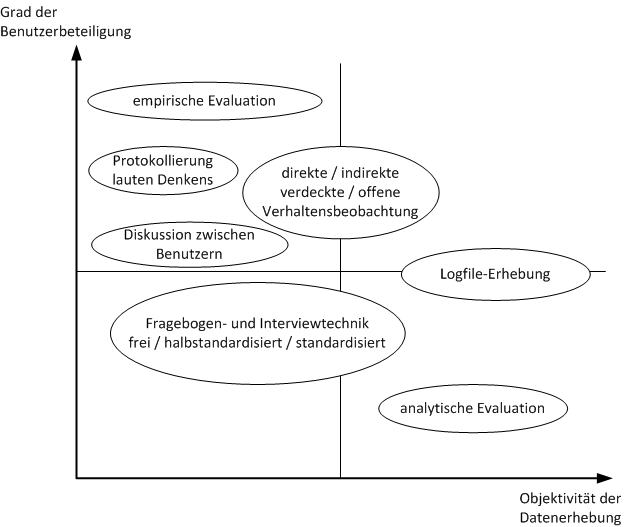
\includegraphics[scale=0.8]{img/Datenerhebungsmethoden_Objektivitaet_Benutzerbeteiligung.png}
  \caption{Vergleich von Erhebungsmethoden aufgrund des Grades der Benutzerbeteiligung und der Objektivität der Methode in Anlehnung an \citep[16]{Hegner2003}}
  \caption*{\textbf{Quelle:} eigene Darstellung}
  \label{fig:erhebungsmethodenObjektivitaetBenutzerbeteiligung}
\end{figure}

Man kann sehen, dass sich die Methoden teilweise nicht genau einer Kategorie zuordnen lassen. Daher wurden zwischen der Subjektivität und der Objektivität noch die Formen der analytischen (leitfadenorientierten) und der empirischen Evaluation eingeführt \citep[vgl.][15]{Hegner2003}.


Im folgenden werden explizit nur die Erhebungsmethoden vorgestellt und eingeordnet, die auch für diese Ausarbeitung zum Einsatz kamen.

\textbf{Logfile-Erhebung}

Eine Methode zur Erhebung objektiver Daten ist die Logfile-Erhebung. Bei der Methode werden die Daten automatisch durch ein Erfassungssystem erhoben. Interaktionen die Benutzer mit dem System erzeugen werden aufgezeichnet. Beispielsweise werden Zeiten zwischen Interaktionen oder die Häufigkeit von Maus- und Tastaturanschlägen gemessen \citep[vgl.][63]{Hegner2003}. 

\textbf{Fragebogen}

Eine subjektive jedoch in Teilen auch objektive Methode ist der standardisierte Fragebogen. Hierbei werden von den Benutzern Meinungen, Erfahrungen und Einschätzungen zum untersuchenden Evaluationsgegenstand eingeholt. Das Ergebnis eines Fragebogens kann durch eine Häufigkeitsauswertung von freien und vorgegebenen Antworten ausgewertet werden. Desto freier die Benutzer antworten können umso vielfältiger wird das Spektrum der Antworten. Auf der anderen Seite sinkt bei steigender Freiheit der Benutzer auch die Bereitschaft zum Antworten und die Konstruktivität der Antworten. Es gibt standardisierte Fragebögen wie den Questionnarie for User Interaction Satisfaction (QUIS), den EN ISO 9241-110 oder den IsoMetrics Fragenbogen, der im folgenden genauer vorgestellt wird \citep[vgl.][Kap. 4.5.1.1]{Hegner2003}.

Der IsoMetrics Fragebogen wurde wie auch der EN ISO 9241-110 Fragebogen basierend auf den sieben Gestaltungsgrundsätzen der DIN EN ISO 9241-110 entwickelt. Sein Fragenkatalog teilt sich daher auch genau in diese sieben Kategorien auf und enthält insgesamt 75 Fragen. Die Fragen lassen sich jeweils auf einer 5-stelligen Skala, von \glqq stimmt nicht \grqq{} bis \glqq stimmt sehr \grqq{}, beantworten. Zusätzlich hat der Befragte bei jeder Frage auch die Möglichkeit \glqq keine Angabe \grqq{} anzukreuzen. In dem Fall wird die Antwort aus der Bewertung herausgenommen. Da es sich im folgenden um eine summative Evaluation handelt, wird der IsoMetrics Fragebogen in seiner Kurzform gewählt. Die Kurzform sieht, im Gegensatz zur Langform, keine freien Felder zur Meinungsäußerung vor \citep[vgl.][Kap. 3.4]{Figl2010}. In Abbildung \ref{fig:isoMetricAntwortschema} wird das Antwortschema des IsoMetric Fragebogens noch einmal gezeigt. Der komplette Fragebogen ist im Anhang ??? zu finden.
\begin{figure}[H]
  \centering
  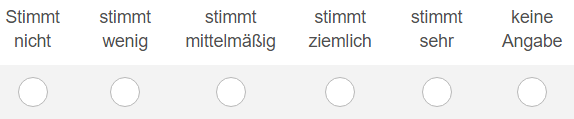
\includegraphics[scale=0.8]{img/IsoMetricAntwortschema.PNG}
  \caption{Antwortschema des IsoMetrics Fragebogens.}
  \caption*{\textbf{Quelle:} eigene Darstellung}
  \label{fig:isoMetricAntwortschema}
\end{figure}


Quelle für den Fragebogen: http://www.isometrics.uni-osnabrueck.de/qn.htm

\subsubsection{Gütekriterien für Erhebungsmethoden}

Die Güte oder auch Qualität einer Erhebungsmethode wird anhand der drei Hauptgütekriterien Objektivität, Validität und Reliabilität bewertet. Darüber hinaus gibt es auch noch weitere Nebengütekriterien (z.B. Normierung, Ökonomie und Nützlichkeit) auf die im Folgenden jedoch nicht genauer eingegangen werden soll \citep[vgl.][Kap. 3.5]{Figl2010}.

Die Objektivität sagt aus, ob ein Testergebnis unabhängig von der Testperson ist. Bedeutet das verschiedene Personen, die gleichen Testergebnisse erzielen \citep[vgl.][Kap. 1]{Himme2007}. Dieses Kriterium wird durch die standardisiert vorgegebenen Antwortmöglichkeiten und die Auswertungsvorschriften für die Ergebnisse gewährleistet \citep[vgl.][Kap. 3.5.1]{Figl2010}.

Die Validität, die angibt inwiefern ein Messinstrument gültig ist bzw. die benötigte Genauigkeit besitzt. Es wird überprüft ob das gemessene, dem entspricht, was gemessen werden soll \citep[vgl][Kap. 1]{Himme2007}. Die Gültigkeit des IsoMetrics Fragebogens wurde bereits bei der Konzeption durch eine Auswahl von theoretisch fundierten Fragen, berücksichtigt \citep[vgl.][Kap. 3.5.2]{Figl2010}.

Als drittes Qualitätsmerkmal wird die Reliabilität herangezogen. Diese beschreibt die Zuverlässigkeit und Stabilität eines Messinstruments. Um eine hohe Zuverlässigkeit bei der Erhebung von Daten zu erreichen, müssen unter anderem gemessene Ergebnisse durch erneutes Messen reproduzierbar sein \citep[vgl.][Kap. 1]{Himme2007}. Die erreichte Reliabilität des IsoMetrics Fragebogens wurde durch \citep[vgl.][2-3]{Gediga1999} mit zufriedenstellend bewertet.

\subsection{Statistische Datenanalyse}
Damit für spätere Auswertungen und Analysen der erhobenen Daten die benutzten Methoden mit denen Daten normalisiert, statistisch bewertet und für grafische Darstellungen aufbereitet werden, klar und verständlich sind werden im Folgenden die Grundbegriffe und weiterreichende Methoden der Statistik, die im Rahmen der Thesis zum Einsatz kommen, vorgestellt und erklärt.

\subsubsection{Bereiche der Statistik}
In der Statistik unterscheidet man zwischen drei grundlegenden Aufgabengebieten. Zum einen die deskriptive Statistik, die sich es sich zur Aufgabe macht Daten komprimiert entweder beschreibend oder grafisch aufzubereiten. Diese Art der Aufbereitung wird häufig zu repräsentativen Zwecken eingesetzt. Dabei kommen verschiedene Diagramme und Tabellen zum Einsatz die dazu dienen zuvor berechnete Durchschnittsgrößen und Kennzahlen der Merkmale und ihrer Ausprägungen darzustellen. Ein zusätzlich wichtiger Aufgabenbereich der deskriptiven Statistik ist die Datenvalidierung. Durch die deskriptive Aufbereitung der Daten lassen sich Fehler leicht aufdecken und gegeben falls beheben. Somit wird der Aufwand für nachträgliche Korrekturen gemindert \citep[vgl.][10\psq]{fahrmeir2016}.

Ein weiterer Teilbereich der Statistik ist die explorative Datenanalyse. Sie bietet Methoden mit denen sich Strukturen und Besonderheiten in den Daten aufdecken lassen. Das führt oft dazu das neue Hypothesen und Fragestellungen hinzu kommen. Daher wird das explorative Vorgehen immer dann verwendet, wenn die Ausgangslage bzw. Fragestellung noch nicht eindeutig ist. Die Exploration wird als Ergänzung der Deskription von Daten angesehen \citep[vgl.][11\psq]{fahrmeir2016}.

Die induktive Statistik ergänzt den dritten Bereich der Statistik. Dort wird über die erhobenen Daten hinweg, mittels Wahrscheinlichkeitstheorie und stochastischer Methoden, Aussagen und Folgerungen geschlossen. Um aussagekräftige Ergebnisse in der Statistik zu erzielen, benötigt man eine klar definierte und sorgfältig strukturierte Versuchsplanung für alle drei Teilgebiet \citep[vgl.][12]{fahrmeir2016}.

\subsubsection{Grundbegriffe}
\textbf{Grundgesamtheit und Stichprobe}

Immer wenn es in der Statistik um die Analyse von Daten geht bei denen die Menge von Bedeutung sind fallen in diesem Zusammenhang Begriffe wie Grundgesamtheit oder Stichprobe. Die Grundgesamtheit hängt von der betrachteten Einheit ab über die man statistische Aussagen treffen möchte und beschreibt die mögliche Menge dieser Einheit. Als Beispiel kann man eine Schule nehmen auf die insgesamt 400 Schüler und Schülerinnen gehen, von denen 250 Jungen und der Rest Mädchen sind. Sollte man nun auswerten wollen wie viele Schüler nun Mädchen bzw. Jungen sind dann besteht die vorliegenden Grundgesamtheit, auf der die statistische Betrachtung basiert, aus allen 400 Schüler und Schülerinnen der Schule.

Geht man nun weiter und möchte seine Erhebung einschränken und nur einen Teil der Grundgesamtheit analysieren, spricht man von einer Stichprobe. Wenn man sich wieder das obige Beispiel nimmt und zum Beispiel wissen will wie viele Jungen im Durchschnitt in der Woche zu spät zum Unterrichtsbeginn kommen, hätte man als vorliegende Stichprobe nur die Jungen der Schule.

\textbf{Einheit, Merkmal und Merkmalsausprägung}

Betrachtet man wieder das Beispiel mit den Schülern, dann ist die Einheit in diesem Kontext ein einzelner Schüler. Sollte man zum Beispiel die Anzahl der Fenster in der Schule ermitteln wollen, dann ist die zu untersuchende Einheit beziehungsweise der Merkmalsträger das Fenster.

Die Eigenschaften einer Einheit nennt man Merkmal. Mögliche Merkmale die man bei einer Analyse von Schülern untersuchen kann sind Körpergröße, Augenfarbe, Haarfarbe oder Geschlecht. Merkmale können verschiedene Merkmalsausprägungen annehmen, die zwischen qualitativen und quantitativen Ausprägungen unterschieden werden. Beispielsweise ist die Körpergröße ein Merkmal mit quantitativen Ausprägungen, in dem Fall sind alle natürlichen Zahlen größer null möglich. Eine qualitatives Merkmal hingegen ist beispielsweise das Geschlecht, das nur zwei Ausprägungen annehmen kann entweder Mann oder Frau.

Grundlegend wird bei Merkmalen und ihren Ausprägungen zwischen drei verschiedenen Skalen zum Messen der Merkmale und ihren Ausprägungen unterschieden. Die Nominalskala stellt das niedrigste Skalenniveau der drei Skalen dar und wird zur Klassifizierung und Darstellung von qualitativen Merkmalsausprägungen verwendet.Merkmale die dieser Skala angehören können lediglich gezählt und in der Häufigkeit ihrer Ausprägungen dargestellt werden.

Das nächst höhere Skalenniveau wird durch die Ordinalskala abgebildet. Beispielsweise gehören Schulnoten (Ausprägungen: sehr gut, gut, befriedigend, ausreichend, mangelhaft und ungenügend) zur Ordinalskala, die neben den Anwendungsgebieten der Nominalskala auch zum Vergleichen von Ausprägungen genutzt werden kann.

Die Intervallskala besitzt nicht nur das höchste Skalenniveau sondern ist auch am vielfältigsten bei der Berechnung von Lageparametern, diese werden im nächsten Abschnitt genauer beschrieben. Zudem lässt sich mit der Intervallskala nicht nur ein Vergleich zwischen Merkmalsausprägungen durchführen sondern auch ein numerischer Unterschied zwischen zwei Ausprägungen ermitteln.


\subsubsection{Lageparameter}
Lageparameter werden in der deskriptiven Statistik zum Beschreiben eines Mittelpunktes innerhalb einer Verteilung\footnote{Verteilung = steht für die relative bzw. absolute Häufigkeit von Merkmalsausprägungen} genutzt. Im folgenden wird auf die als Lageparameter zählenden Größen Modus, Median und arithmetisches Mittel genauer eingegangen.

Als ersten Lageparameter betrachten wir den Modus, der angibt welche Merkmalsausprägung in einer Verteilung am häufigsten vorkommt. Als Beispiel nehmen wir eine Befragung bei der eine Stichprobe von 500 Probanden nach ihrer Lieblingsjahreszeit befragt werden. Das Ergebnis der Erhebung ist:
\begin{center}
\begin{tabular}{r|c|c|c|c} 
\textbf{Jahreszeit} & Frühling & Sommer & Herbst & Winter \\ \hline
\textbf{Anzahl Probanden} & 110 & 205 & 85 & 110\\
\end{tabular}
\end{center}
Will man nun den Modus bestimmen sucht man unter den Merkmalsausprägungen die Ausprägung mit den meisten Probanden, in diesem Fall ist das der Sommer.

Im nächsten Schritt wollen wir anhand eines Beispiels den Median berechnen. Da der Median nur auf Ordinalskalen oder Intervallskalen angewandt werden kann ist das vorherige Beispiel nicht für den Median geeignet. Das vorliegende Beispiel ist lediglich nominal skaliert.
Um ein Beispiel für den Median zu finden betrachten wir das Alter von 10 zufällig ausgewählten Probanden die im ersten Semester Biologie studieren. Die Stichprobe sieht wie folgt aus:
\begin{center}
\begin{tabular}{r|c|c|c|c|c|c|c|c|c|c} 
\textbf{Rang} & 1 & 2 & 3 & 4 & 5 & 6 & 7 & 8 & 9 & 10 \\ \hline
\textbf{Alter} & 20 & 20 & 22 & 23 & 23 & 23 & 25 & 25 & 25 & 26\\
\end{tabular}
\end{center}
Wie sich aus der Tabelle ablesen lässt gibt es 2 x 20, 1 x 21, 3 x 23, 3 x 25 und 1 x 26 als Alter der befragten Probanden. Um den Median nun zu bestimmen ordnet man die erhobenen Daten nach ihrer Größe (ist in der obigen Grafik schon geschehen) und wählt den mittleren Wert dieser sortierten Reihe. In diesem Beispiel gibt es zwei mittlere Werte die in Frage, da die Anzahl $N$ der befragten Probanden gerade ist. Bedeutet für diesen Fall, dass man diese beiden Merkmalsausprägungen addiert und anschließend durch zwei dividiert, um den Median zu erhalten. Die konkrete Rechnung dazu sieht folgendermaßen aus: $Median = \frac{23 + 23}{2} = 23$.

Der letzte Lageparameter der immer dann angewendet werden kann, wenn eine Intervallskala vorliegt ist das arithmetische Mittel. Das arithmetische Mittel, auch bekannt als Mittelwert, gibt den Durchschnittlichen Wert aus einer Datenmenge mit $N$ Merkmalsausprägungen an. Der Mittelwert $\bar{x}$ ergibt sich aus der Summe aller Merkmalsausprägungen geteilt durch die Anzahl $N$ Werte. Nimmt man das obige Beispiel um den Mittelwert zu berechnen sieht die Rechnung wie folgt aus: \\
$Mittelwert = \frac{\sum \limits_{i=1}^N X_i}{N} = \frac{20\,+\,20\,+\,22\,+\,23\,+\,23\,+\,23\,+\,25\,+\,25\,+\,25\,+\,26}{10} = 23,2 Jahre$. Die Berechnung hat ergeben, dass die Erstsemester Biologie Studenten im Schnitt 23,2 Jahre alt sind.

\subsubsection{Dispersionsparameter}
Die nächste Sektion beschäftigt sich mit den Dispersionsparametern, die immer dann zum Einsatz kommen wenn es darum geht ein Maß für die Streuung von Messwerten um ein Zentrum zu ermitteln, zu denen unter anderem die Spannweite, die Varianz und die Standardabweichung gehören.

\textbf{Spannweite}

Die Spannweite kommt immer dann zum Einsatz wenn man wissen möchte wie weit der größte (Maximum) und der kleinste (Minimum) Wert einer Messreihe auseinander liegen. Es wird der kleinste Wert vom größten Wert der Messung subtrahiert und man erhält die Spannweite. Dazu eine Beispielrechnung mit der zuletzt aufgestellten Messreihe: $Spannweite = 26 - 20 = 6$, damit ist die Spannweite zwischen dem jüngsten und dem ältesten Studenten der Untersuchung 6 Jahre.

\textbf{Varianz}

Wenn es in den späteren Auswertungen darum geht herauszufinden wie weit die Messwerte durchschnittlich von dem arithmetischen Mittel abweichen, berechnet man die Varianz. Die Varianz ist ein Maß, um die Streuung von Messwerten um den Mittelwert zu bestimmen. Für die Varianz wird bei empirischen Erhebungen und auch für unsere weiteren Rechnungen als Platzhalter $s^2$ verwendet. Die Berechnung startet damit, dass die quadrierte Abweichung jedes einzelnen Messwertes vom Mittelwert aufsummiert und anschließend durch die Anzahl der Messwerte dividiert werden. Das Quadrat wird aus dem Grund verwendet, dass negative Abweichungen, die aus der Differenz von $Mittelwert\:\bar{x} - Messwert\:X $ entstehen können, nicht die positiven Abweichungen aufheben und das Ergebnis verfälschen. Die entsprechende Rechnung zum obigen Beispiel: \\
$s^2 = \frac{\sum \limits_{i=1}^N (X_i\,-\,\bar{x})^2}{N} = \frac{(20\,-\,23,3)\:+\:(20\,-\,23,2)\:+\:...\:+\:(26\,-\,23,2)}{10} = 3,96$. 

Das Ergebnis von 3,96 ist nun ein Maß, das die Streuung um den Mittelpunkt angibt, jedoch wäre es falsch diesen Wert eins zu eins als absolute Abweichung zu nehmen, da sich in der Rechnung durch das Quadrieren das Endergebnis ebenfalls als Quadrat der eigentlichen Abweichung ansehen lässt.

\textbf{Standardabweichung}

Um diesem Berechnungsproblem aus dem Weg zu gehen, gibt es die Standardabweichung $s$ als weiteren Dispersionsparameter, den man anstelle der Varianz häufig in der Statistik einsetzt. Die Standardabweichung bildet die Durchschnittliche Abweichung der Messwerte um den Mittelwert besser ab als die Varianz, da hier das Quadrat das beim berechnen der Varianz am Ende wieder durch ziehen der Quadratwurzel eliminiert wird. Bedeutet im Klartext, dass die Berechnung der Standardabweichung der der Varianz gleicht, bis auf die Quadratwurzel am Ende. Somit muss man um $s$ für das Beispiel zu berechnen die Wurzel von $s^2$ ziehen. Dann sieht die Rechnung wie folgt aus: $s = \sqrt{s^2} = \sqrt{3,96} = 1,99$. Interessant wird dieser Parameter dann, wenn man wissen möchte wie aussagekräftig der Mittelwert einer Messreihe wirklich ist. Um das näher zu zeigen wird im folgenden eine weitere Messreihe zu Erstsemester Biologie Studenten mit Zehn Probanden aufgestellt.
\begin{center}
\begin{tabular}{r|c|c|c|c|c|c|c|c|c|c} 
\textbf{Rang} & 1 & 2 & 3 & 4 & 5 & 6 & 7 & 8 & 9 & 10 \\ \hline
\textbf{Alter} & 18 & 18 & 19 & 22 & 23 & 23 & 25 & 26 & 28 & 29\\
\end{tabular}
\end{center}
Schaut man sich nun die Mittelwert beider Messreihen an stellt man fest das sie mit 23,2 Jahren identisch sind, somit könnte man davon ausgehen das sich die Messwerte sehr ähneln müssen. Genau an dieser Stelle muss man genau hinsehen und sollte von der Standardabweichung Gebrauch machen, um diese Aussage genauer zu validieren. Denn wenn man für beide Messungen die Standardabweichung $s$ berechnet merkt man, dass die Abweichung der ersten Erhebung, wie vorher schon kalkuliert, bei 1,99 liegt, jedoch die Standardabweichung der zweiten Messreihe bei etwa 3,84 liegt und damit fast doppelt so groß ist. Für dieses Beispiel wird nun ersichtlich das sich die Messreihen wohl doch nicht so ähneln wie anfänglich gedacht und die durchschnittliche Streuung um den Mittelwert fast doppelt so groß ist. Das heißt man sollte in diesem Fall vorsichtig sein, vergleichende Aussagen mit Hilfe des arithmetischen Mittels zu treffen, ohne weitere Parameter wie die Standardabweichung mit hinzuzunehmen.

\subsubsection{Studentsche T-Test und $Chi^2$ Unabhängigkeitstest}

\subsection{Kosten-Nutzen-Analyse}
Die Kosten-Nutzen-Analyse (KNA) ist eine Methode mit der durch den Vergleich von Kosten und Nutzen eine objektive Aussage über die Wirtschaftlichkeit eines Projektvorhabens getroffen werden kann. Auf der einen Seite werden die Kostenpunkte eines Projektes identifiziert und quantifiziert. Auf der anderen Seite werden jegliche zu erwartende Effizienzpotential, die aus dem Projektvorhaben resultieren, betrachtet und für einen Vergleich monetarisiert. Die KNA ist für verschiedenste Personen eines Projektes interessant. Zum Beispiel sind der Auftraggeber und Investoren daran gelegen, dass sich das Projekt und die damit entstehenden Kosten nach einer gewissen Zeit amortisieren und ein positives Ergebnis erzielt wird. Gerade in der Planungsphase eines Projekts können Projektbeteiligte mit Hilfe der KNA die positiven und negativen Effekte eines Projekts besser abschätzen und so gezielter und effektiver planen und agieren. Im Folgenden wird auf Grund des Projektumfangs meiner Bachelor Thesis nur von einer minimalistischen Form der KNA Gebrauch gemacht. In der späteren Analyse werden bewusst einige Kosten und Nutzen, die entweder nicht klar identifizierbar sind oder wenn erfassbar dann nur in Verbindung mit übermäßigem Aufwand, vernachlässigt. 

Ein Bestandteil der KNA, der im oberen Teil schon kurz erwähnt wurde, ist der Amortisationszeitpunkt des zu überprüfenden Projektes, also der Zeitpunkt an dem die Summe der Kosten und der Nutzen gleich null sind. Dieser Zeitpunkt wird auch als Break-Even-Point bezeichnet. Umso näher der Break-Even-Point am Startzeitpunkt des Projekts liegt desto höher ist dessen Wirtschaftlichkeit einzuschätzen.

Ein weitere Begriff der im Zusammenhang mit der KNA häufig fällt ist das Effizienzpotential. Dies sagt aus, dass der Nutzen eines Projekts ein gewisses Potential besitzt. Jedoch wird dieser Nutzen relativiert, da er in Wirklichkeit noch nicht realisiert wurde und sich durch die Veränderung von Einflussfaktoren zukünftig noch ändern kann. Die Kosten-Nutzen-Analyse \glqq [...] stellt das wohl bekannteste wirtschaftlichkeitsanalytische Verfahren für den öffentlichen Sektor dar\grqq{} \citep[1]{Hanusch2011}. Es gibt den Projektplanern aber nie eine 100\% Sicherheit über das tatsächliche Endergebnis eines Projektes.

